\documentclass[11pt]{article}
\usepackage{mystyle}

\title{Notes on x-ray data}
\author{Scott Trinkle}
\date{Last edited: \today}

\newsavebox{\largestimage}

\begin{document}

\maketitle

\section{Introduction}

The aim of these notes is to discuss and characterize the post-processing steps
involved in preparing the reconstructed $\upmu$CT data for further analysis.

\subsection{Data size reduction}
The full resolution (1.2 $\upmu$m isotropic) $\upmu$CT data\footnote{In these
notes, I refer to what I am told is the ``best'' $\upmu$CT dataset that has a
corresponding DW-MRI volume, located in
\texttt{/data\char`_raf/2017\char`_07\char`_22\char`_WholeMouseMRI\char`_5x\char`_2k\char`_phase35cm\char`_gap31\char`_exp30\char`_newfocus/
  recon\char`_flatcorr\char`_1x/recon\char`_crop\char`_8/} \newline on globus.}
is reconstructed with 32-bit float precision, with an image size of
11982$\times$11982$\times$13781 voxels. A single slice is thus \textapprox 548
MB and the full volume is \textapprox 7.5 TB. The first family of
post-processing steps attempt to reduce the data size. First, each slice is
cropped to a 10096$\times$6720 voxel field of view that just includes the extent
of the brain volume. Next, the data values are rescaled from 32-bit floating
point values to 8-bit unsigned integers.\footnote{I am still communicating with
  Raf to understand how he does this rescaling. He claims that the rescaling
  causes the denoising, but I am able to better replicate his results after
  Gaussian filtering as well.} These two operations reduce a single slice to
\textapprox 68 MB, a reduction of \textapprox 87\%. A comparison of the pre- and
post-processed data is shown in Figure~\ref{fig:datacomp}.



% \begin{figure}[h]
%   \centering
%   \savebox{\largestimage}{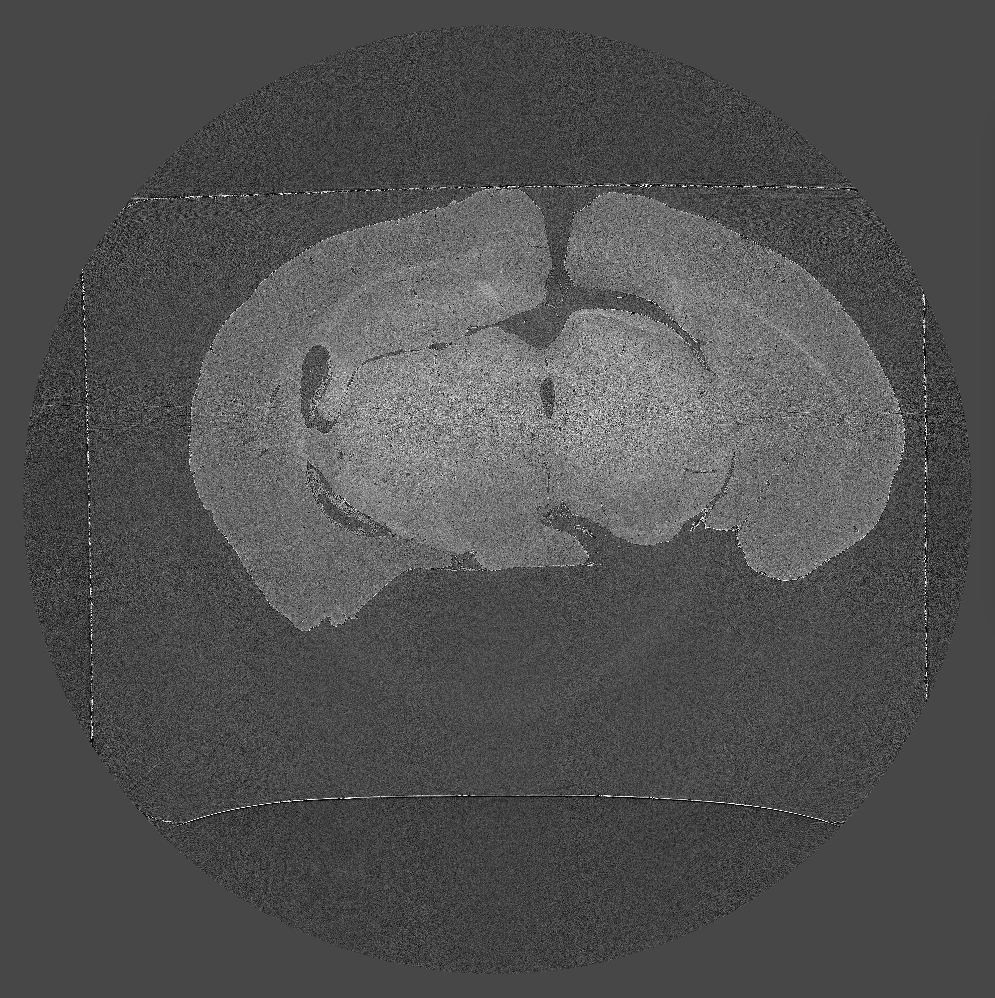
\includegraphics[width=0.432\linewidth]{figs/recon_06250}}
%   \begin{subfigure}[t]{0.48\textwidth}
%     \centering
%     \usebox{\largestimage}
%   \end{subfigure}
%   \hspace{1em}
%   \begin{subfigure}[t]{0.48\textwidth}
%     \centering
%     \raisebox{\dimexpr.5\ht\largestimage-.5\height}{%
%       \includegraphics[width=0.9\linewidth]{figs/recon_crop_8_06250}}
%   \end{subfigure}
%   \vspace{1em}
%   \begin{subfigure}[b]{0.48\textwidth}
%     \centering
%     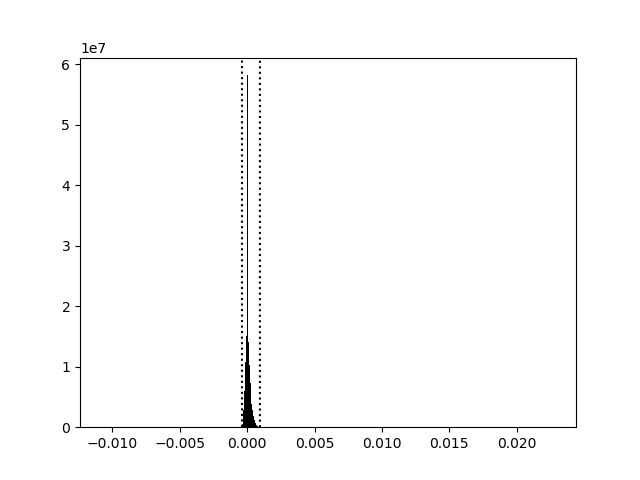
\includegraphics[width=0.9\linewidth]{figs/recon_orig_hist}
%     \caption{Raw 32-bit slice. Display: [-4.95e-4, 1.9e3]}
%   \end{subfigure}
%   \hspace{1em}
%   \begin{subfigure}[b]{0.48\textwidth}
%     \centering
%     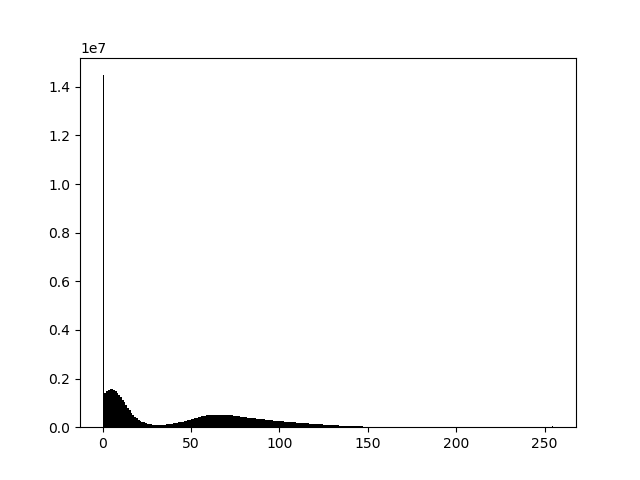
\includegraphics[width=0.9\linewidth]{figs/recon_crop8_hist}
%     \caption{Cropped, 8-bit, denoised slice}
%   \end{subfigure}
%   \caption{Comparison of raw and processed reconstructed data.}
%   \label{fig:datacomp}
% \end{figure}

% \begin{figure}[h]
%   \centering
%   \begin{subfigure}[b]{0.48\textwidth}
%     \centering
%     \includegraphics[height=6cm]{figs/composite}    
%   \end{subfigure}
%   \hspace{1em}
%   \begin{subfigure}[b]{0.48\textwidth}
%     \centering
%     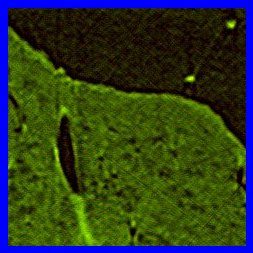
\includegraphics[height=6cm]{figs/composite_zoom}    
%   \end{subfigure}
%   \captionsetup{width=0.9\textwidth}
%   \caption{Composite of custom-cropped (green) vs. globus-cropped (red) slice. From visual
%     inspection, there seems to be agreement within a few voxels at most.}
%   \label{fig:composite}
% \end{figure}


\begin{center}
  \captionsetup{width=0.9\textwidth}
  \captionof{figure}{Caption}
  \begin{longtable}{M{0.15\textwidth} M{0.15\textwidth} M{0.3\textwidth} M{0.3\textwidth}}
    Image & ACC & 32-bit ODF & 8-bit ODF\\
    test & acc & \im{0.3}{\odfpath{32}{1}} & \im{0.3}{\odfpath{8}{1}}\\
    test & acc & \im{0.3}{\odfpath{32}{2}} & \im{0.3}{\odfpath{8}{2}}\\
    test & acc & \im{0.3}{\odfpath{32}{3}} & \im{0.3}{\odfpath{8}{3}}\\
    test & acc & \im{0.3}{\odfpath{32}{4}} & \im{0.3}{\odfpath{8}{4}}\\
    test & acc & \im{0.3}{\odfpath{32}{5}} & \im{0.3}{\odfpath{8}{5}}\\
    test & acc & \im{0.3}{\odfpath{32}{6}} & \im{0.3}{\odfpath{8}{6}}\\
    test & acc & \im{0.3}{\odfpath{32}{7}} & \im{0.3}{\odfpath{8}{7}}\\
    test & acc & \im{0.3}{\odfpath{32}{8}} & \im{0.3}{\odfpath{8}{8}}\\
    test & acc & \im{0.3}{\odfpath{32}{9}} & \im{0.3}{\odfpath{8}{9}}    
  \end{longtable}
\end{center}
% \bibliographystyle{ieeetr}
% \bibliography{bitdepth}

\end{document}
